\documentclass[12pt, dvipsnames, svgnames, x11names,]{article}

\usepackage{xcolor}
% URLs and hyperlinks ---------------------------------------
\usepackage{hyperref}
\hypersetup{
	colorlinks=true,
	linkcolor=NavyBlue,
	filecolor=magenta,      
	urlcolor=blue,
}
\usepackage{xurl}
%---------------------------------------------------
\usepackage[inline]{enumitem}
\usepackage{graphicx}
\usepackage{multirow}
\usepackage{float}
\renewcommand{\arraystretch}{1.40}

% adjust a verrrrry big table -------------------------------
\usepackage{adjustbox}
% -----------------------------------------------------------

\usepackage{array}
% center the p columns and m --------------------------------------------------------------
\newcolumntype{P}[1]{>{\centering\arraybackslash}p{#1}}
\newcolumntype{M}[1]{>{\centering\arraybackslash}m{#1}}
% -------------------------------------------------------------------------------------------------------------

% price
\usepackage{marvosym}
% ----------

\usepackage{xepersian}
\settextfont{Arial}
\setdigitfont{Arial}

\begin{document}
	\begin{titlepage}
		\centering
		\vspace{1cm}
		{\Huge {\textbf{رگرسیون خطی چند متغیره}}\par}
		\vspace{15mm}
		\vspace{16mm}
		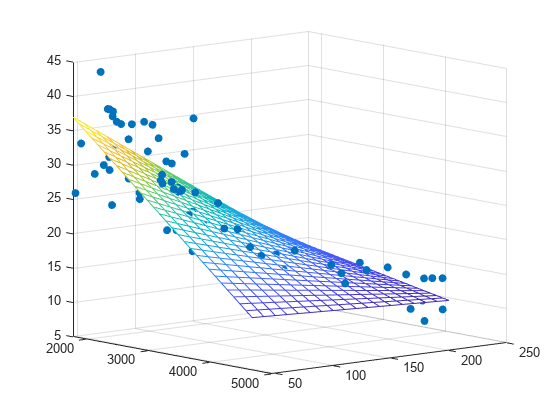
\includegraphics[width=14cm]{images/EstimateMultipleLinearRegression} \par
		\vfill \par	\vfill
		\vspace{16mm}
		{\normalsize	سیدمحمدحسین هاشمی  4022363143 \par}
		
		{\normalsize	سیدحسین حسینی  4012363238 \par}
		\vspace{1cm}
		{\large آبان ۱۴۰۲\par}
	\end{titlepage}
	\tableofcontents
	\newpage
	
	
	\section{پکیج های استفاده شده}
	
		{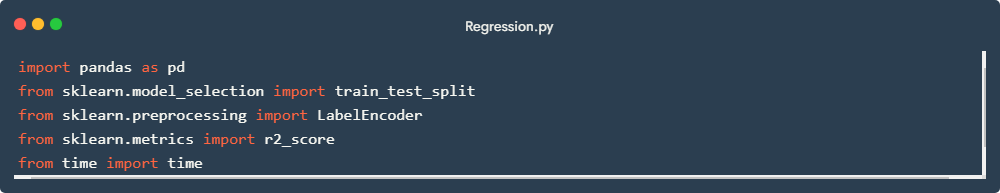
\includegraphics[width=14cm]{images/libraries}}
	
		\begin{itemize}
			\item 
			{\Large \lr{pandas}:}
			{\small برای ایجاد \lr{dataframe} .و تقسیم بندی داده ها مورد استفاده قرار می‌گیرد}
		
				
			\item 
			{\Large \lr{sklearn}:}
			{\small برای تقسیم بندی، دسته بندی داده‌ها و محاسبه خطا \lr{R Squared (R2)}}
		
			\item 
			{\Large \lr{time}:}
			{\small برای محاسبه زمان اجرای الگوریتم}
		
		\end{itemize}
	
				
	
	\section{آماده سازی برای شروع}
	
		{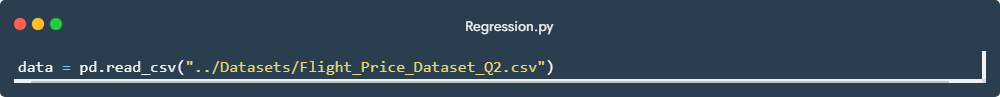
\includegraphics[width=14cm]{images/code01}} \par
		{\normalsize
		 	ساخت دیتافریم با متد \lr{read\_csv} پکیج \lr{pandas}
		}
	
	
	\section{تبدیل داده‌های دسته‌ای}
	
		{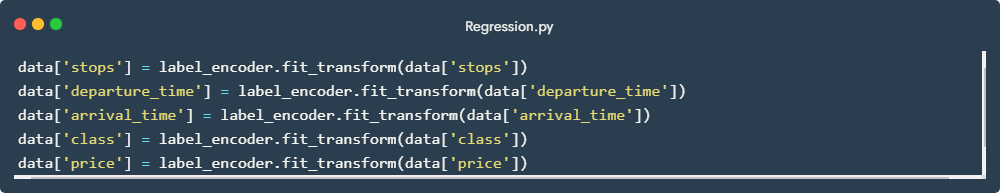
\includegraphics[width=14cm]{images/code02}} \par
		{\normalsize
			تبدیل داده‌های دسته‌ای به داده‌های قابل پردازش در ستون‌های:
		} \par
		\begin{itemize}
			
			\item 
			{\normalsize \lr{departure\_time}}
			
			\item 
			{\normalsize \lr{stops}}
			
			\item 
			{\normalsize \lr{arrival\_time}}
			
			\item 
			{\normalsize \lr{class}}

			
		\end{itemize}
	
	
	
	\section{جدا سازی داده‌ها}
	
		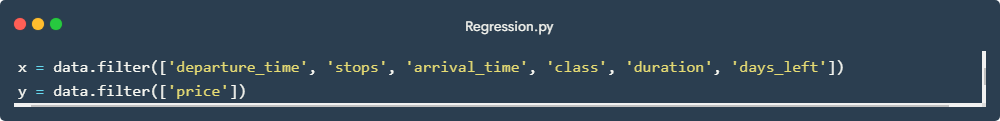
\includegraphics[width=14cm]{images/code03} \par
		{\normalsize 
			جدا سازی داده‌های ورودی و خروجی
		}
		
	
	
	\section{مقیاس کردن داده‌ها}
	
		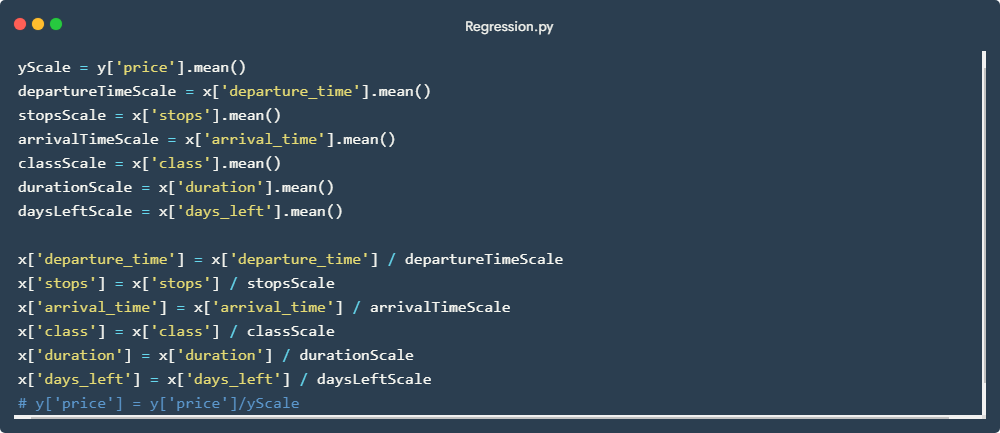
\includegraphics[width=14cm]{images/code04} \par
		{\normalsize 
			مقیاس کردن داده‌های ورودی برای پردازش صحیح الگوریتم.
			تقسیم هر مقدار از یک دسته به میانگین کل داده‌های آن دسته.
		}		
	
	
	
	\section{تقسیم بندی داده‌ها}
	
		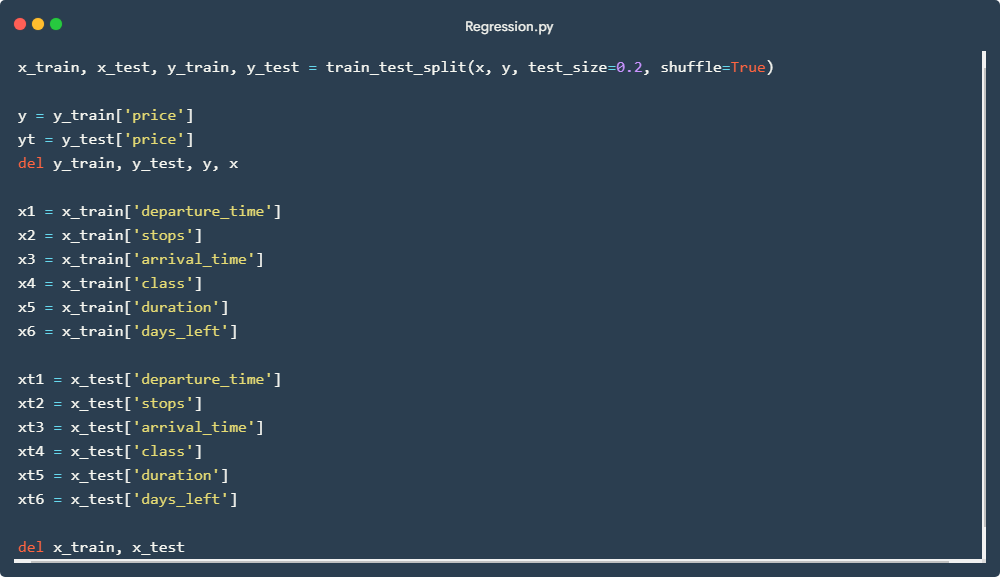
\includegraphics[width=14cm]{images/code05} \par
		{\normalsize 
			تقسیم بندی داده ها با استفاده از \lr{LabelEncoder} در \lr{sklearn} (روش گفته شده در قسمت مقدمات)
		}
	
	
	
	\section{آماده سازی پردازش} \label{pre_proccess}
	
		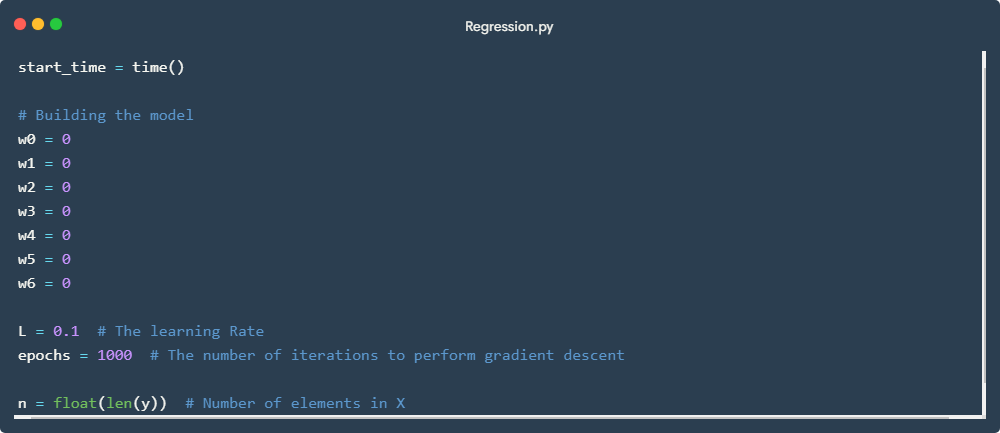
\includegraphics[width=14cm]{images/code06} \par
		{\normalsize 
			مقدار \lr{start\_time} را ایجاد و به متغییرهای رابطه به طور پیش فرض مقدار 0 را انتصاب می‌دهیم.
			
			مقدار \lr{L} همان ضریب یادگیری و \lr{epochs} تعداد تکرار الگوریتم گرادیان کاهشی (\lr{Gradient Descent}) از مبحث کاهش شیب می‌باشد.
			مقدار \lr{n} نیز تعداد داده‌هاست.
		}
		
			
		
		
	\section{پردازش اصلی (یافتن ضرایب)}
		
		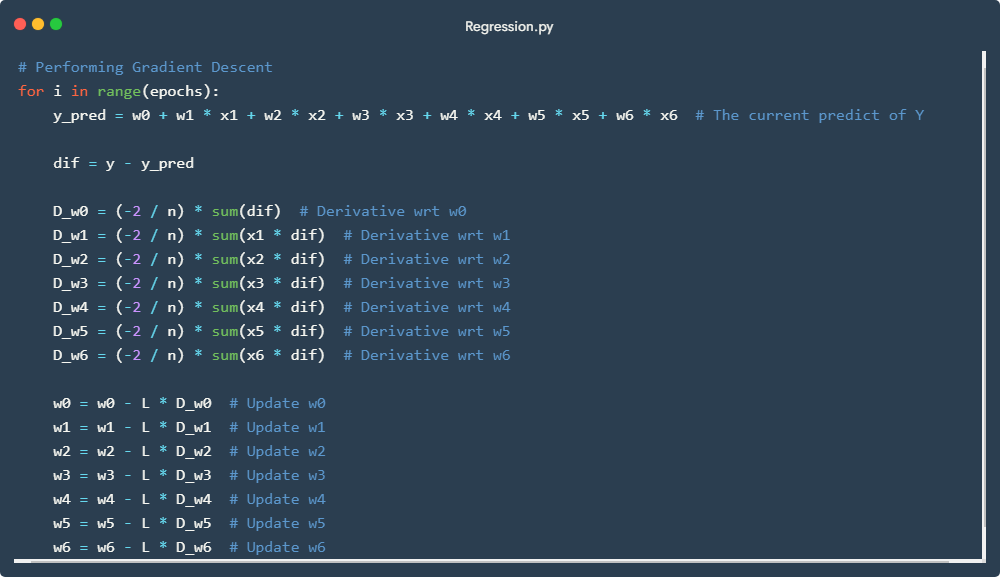
\includegraphics[width=14cm]{images/code07} \vspace{2mm} \par
		{\normalsize 
			با استفاده از فرمول زیر
			\[ D_m = \frac{1}{n} \sum_{i=0}^n 2(y_i - (mx_i + c))(-x_i) \] \[ D_m = \frac{-2}{n} \sum_{i=0}^n x_i(y_i - \bar y_i) \]
			
			در هر بار اجرا برای هر متغیر فرمول فوق محاسبه و بر اساس ضریب یادگیری تعیین شده در قسمت \ref{pre_proccess} مقدار متغییرها مجددا تائین می‌شود.
		}
	
		
	
	
	\section{محاسبه خطا و تحویل خروجی}
	
	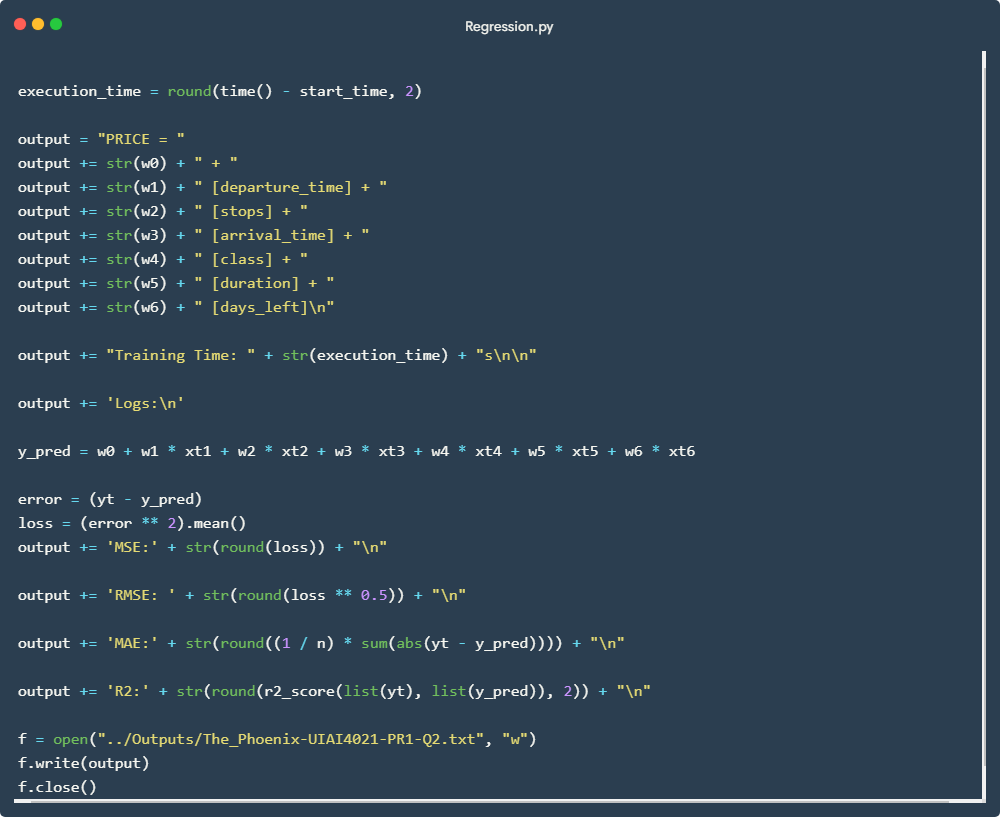
\includegraphics[width=14cm]{images/code08} \par
	{\normalsize 
		در این بخش از همزمان با استفاده از مقادیر تستی مقادیر خطا را تحت معیار های متختلف حساب و همزمان خروجی را تحویل می‌دهیم.
		
		معیارهای سنجش خطا استفاده شده به ترتیب:
	}
	\begin{itemize}
		
		\item 
		{\Large \lr{Mean Squared Error (MSE)}:} \par
		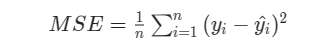
\includegraphics[width=8cm]{images/MSE}
		
		\item 
		{\Large \lr{Root Mean Squared Error (RMSE)}:} \par
		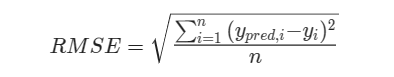
\includegraphics[width=8cm]{images/RMSE}
		
		\item 
		{\Large \lr{Mean Absolute Error (MAE)}:} \par
		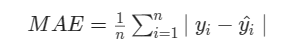
\includegraphics[width=8cm]{images/MAE}
		
		\item 
		{\Large \lr{R Squared (R2)}:} \par
		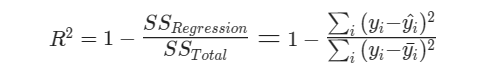
\includegraphics[width=8cm]{images/R2}
		
	\end{itemize}
	
	
	
	
	\section{منبع} \label{resource}
	
	\begin{itemize}
		
		\item 
		\textbf{\lr{https://github.com/chasinginfinity/ml-from-scratch/tree/master}}
		
		
	\end{itemize}
	
\end{document}